

\subsection{Scheduling CP}

\begin{center}
    \texttt{cumulative($[s_1,..., s_n], [d_1, ..., d_n], [e_1, ...,
    e_n], [c_1, ..., c_n], C$)}
\end{center}

\begin{itemize}
    \item $\forall_i: s_i + d_i = e_i$
    \item $\forall_t: \sum_{s_i \leq t < e_i} c_i \leq C$
\end{itemize}

\subsubsection{Sweep line algorithm}
It's use to compute the cumulated
profile and check that it does not exceed the capacity.


\begin{enumerate}
    \item \begin{tabular}{m{5cm}m{10cm}}
            \begin{itemize}
                \item One time point for start $(start, +capa)$
                \item One time point for end $(start, -capa)$ 
            \end{itemize}&
                    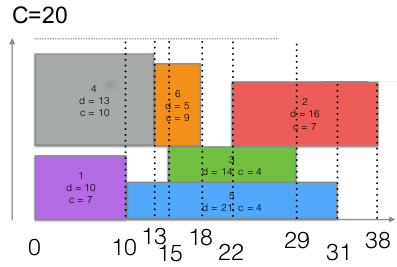
\includegraphics[width=7cm]{sweepLine}
                \end{tabular}


            \item \begin{tabular}{m{5cm}m{8cm}}
                    \begin{itemize}
                        \item Sort time points
                    \end{itemize}
                    &

                    (0,+7), (0,+10), (10,-7), (10,4), (13,-10), (13,9), (15,4), (18,-9), (22,7), (29,-4), (31,-4), (38,-7)
                \end{tabular}

            \item \begin{tabular}{m{5cm}m{10cm}}
                    \begin{itemize}
                        \item Sweep-line(t) = height of the profile at time $t$.
                    \end{itemize}
                    &
                    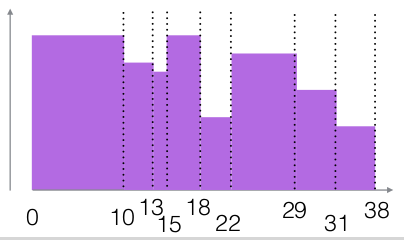
\includegraphics[width=7cm]{sweepLine2}
                \end{tabular}

                \begin{lstlisting}[mathescape]
input = eventQueue$[(time,c)]$
t = input.head.time   // Current time of the sweep line
h = 0                 //  current capacity of the sweep line 

while (input.nonEmpty) {
    while (input.nonEmpty && input.head.time == t){
    (time,c) = input.dequeue
    h = h + c
    }
    add (t,h) to the profile
    t = input.top.time
}
            \end{lstlisting}
    \end{enumerate}


\subsubsection{Optimistic Resource Profile}

\begin{tabular}{m{11cm}m{6cm}}
The optimistic resource profile is built based on the
\textbf{mandatory parts} which is the time where the activity will
use the resource whatever it final position.
&
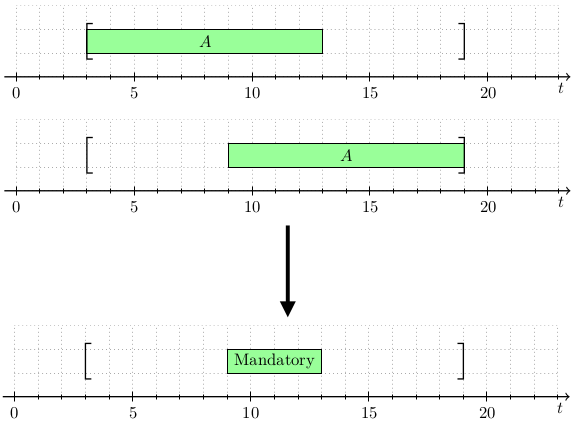
\includegraphics[width=4cm]{mandatory}
\end{tabular}

\begin{itemize}
    \item \textbf{Update minimum start time} at the earliest
        time such that it is not in conflict with the optimistic
        resource profile.

        \paragraph{Time complexity}: $O(n)$ per task since recource
        profile has $O(n)$ intervals. So, $O(n^2)$ overall.
\end{itemize}


\subsection{Large Neighbors Search}



